\documentclass{article}
\usepackage[a4paper, margin=2cm]{geometry} 
\usepackage[T1]{fontenc} %lädt Deutsche schriftzeichen
\usepackage{amssymb}%für Mathe
\usepackage{setspace} %für Zeilen Abstand 
\usepackage[none]{hyphenat} % Silbentrennung deaktivieren 
\usepackage{fancyhdr}%Kopf und Fußzeile: https://de.overleaf.com/learn/latex/Headers_and_footers
\usepackage{graphicx}%Zum Bilder einfügen
\usepackage[dvipsnames]{xcolor}%Für Farbe 
\usepackage{wrapfig}
%\usepackage[document]{ragged2e}%für Blocksatz
\usepackage[ddmmyyyy]{datetime}%zum bearbeiten vom Datungs Format
\usepackage{eurosym}%für \Euro / \euro
\usepackage{hyperref}
\usepackage{listings}%Code meines wissens nach
\usepackage{tcolorbox}%textboxen erweiterung

\setcounter{secnumdepth}{5}
\setcounter{tocdepth}{5}

\makeatletter
\newcommand\subsubsubsection{\@startsection{paragraph}{4}{\z@}{-2.5ex\@plus -1ex \@minus -.25ex}{1.25ex \@plus .25ex}{\normalfont\normalsize\bfseries}}
\newcommand\subsubsubsubsection{\@startsection{subparagraph}{5}{\z@}{-2.5ex\@plus -1ex \@minus -.25ex}{1.25ex \@plus .25ex}{\normalfont\normalsize\bfseries}}
\makeatother

\newcommand{\authoren}{Niklas Hainz}
\newcommand{\Thema}{Spiel Projekt}
\newcommand{\Fach}{Praktische Informatik}
\newcommand{\Zeilenabstand}{1.2}
\newcommand{\Inhaltsverzeichnisname}{Inhaltsverzeichnis}


\newcommand{\absatz}{5mm}
\newcommand{\Blocksatz}{\justifying}
\newcommand{\strich}{\vspace{\absatz}\hrule\vspace{\absatz}} 


\title{\Thema}
\author{\authoren}
\date{\today}


\setlength{\parindent}{0cm} %deaktiviert die Automatische Einrückung am Anfang des Dokumentes 
\renewcommand{\contentsname}{\Inhaltsverzeichnisname}
\renewcommand{\dateseparator}{.}







\begin{document}
\begin{spacing}{\Zeilenabstand}
\maketitle
\begin{center}
    \vspace{-\absatz}
    \Fach
\end{center}
\thispagestyle{empty}
\newpage

\pagestyle{fancy}
\fancyhead[L]{\authoren}
\fancyhead[C]{\Thema / \Fach}
\fancyhead[R]{\today}
\fancyfoot[C]{\thepage}
\fancyfoot[R]{}

\pagenumbering{roman}
\setcounter{page}{1}
\tableofcontents
\listoffigures


\newpage

\pagenumbering{arabic}
\setcounter{page}{1}


%%% Document start %%%

\section{Einleitung}

Bubble Bobble ist einen Sehr am Orginal (Bubble Bobble aus dem Jahr 1986 entwickelt von taito) insperierten
spiel das diese Nachahmt. Es geht darum Gegner in einem Stationären Level zu vernichten dies 
Kann man mit Blasen als Spieler machen. 

\section{Planung}

\subsection{Produktskizze}

Das geplante Spiel soll den gleichen Aufbau und Ablauf wie das Spiel "Bubble Bobble" haben: Das Spiel besteht aus mehreren Leveln, welche alle eine Verschiedene Anzahl und Typen an Gegnern beinhalten. Diese Gegnere müssen alle Besigt werden um in das nächste Level zu kommen. Die Gegner sind besiegbar mit Blasen die vom Spieler aus geschoßen werden können.


\subsubsection{Ziel des Spieles}

Das Ziel des Spieles ist es alle Level zu bestehen.


\subsubsection{Genre des Spiels}

Das Spiel ist das Genre Jump `n' Run 

\subsubsection{Grobe Struktur der Benutzeroberfläche}

Oben in der Mitte soll immer der Highscore und der Score vom ersten Spieler links und den Score von dem Zweiten Spieler unten Links sollte noch die Leben in form von Blasen angezeigt werden.

\subsubsection{Aufgaben und Vorgehen des Spielers}

Der Spiel muss alle Gegner besiegen bis er ins nächste Level kommt. 

\subsubsection{Spielende}

Das Spielende tritt ein wenn Spieler eins und Spieler zwei keine Leben mehr haben, dann wird ein ``Game over'' screen eingeblendet.

\subsection{Prototypen}

\begin{figure}[h]
    \includegraphics[scale=0.5]{media/Bubble_bobble_remake_proto.png}
    \label{Bubble_Bobble_remake_Proto}
\end{figure}

Die Roten Rechtecke in der Mitte sind gegner. Das blaue und das Grüne Rechtecke sind Spieler eins(Grün) Spieler zwei(Blau).Die Rechtecke links und Rechts sind für ein Bonus Leben. Oben in der Mitte ist der Highscore der, der gleiche ist wie der höchste Spieler punktzahl oder wenn der einer der Aktuellen spielern ein Höhren Highscore hat dann wird dieser ersetzt und Geupdate.


\subsubsection{Spielbeginn}

Zu Spiel beginn muss entweder eine virtuelle Münze eingeworfen werden(Start Taste) oder das Spiel Starte direkt 

\subsubsection{Typische Szene im Spiel}

Spieler kämpt gegen Gegner um ins Nächste Level zu kommen. Ggf. Zwei Spieler.

\subsubsection{Spielende}

Spiel ende Trifft eine wenn beide Spieler keine Leben mehr haben. Dann würde der  ``Game Over''  Screen eintreten 

\subsection{Versionierung}

Versionierung mit Git.
Plannung sind mindesten 20 Level wünschenswert währen mehr bis alle 100 und einführung von den Bonbons als Powerups auch hier wäres wünschens wert wenn es noch mehr Items hinzugefügt werden.
Selbst erstelle Sprites. 

\newpage



\section{Entwurf}

\subsection{Struktogramm einer   Methoden}

\begin{figure}[h]
    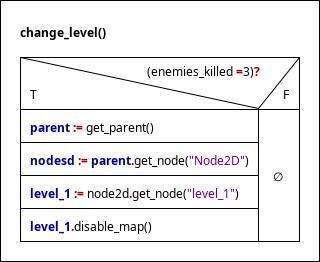
\includegraphics[scale=0.4]{media/change_level.png}
    \caption{Struktogramm Change Level}
\end{figure}

\section{Durchführung}

\subsection{Beschreibung Ablauf }

\subsubsection{Ideenfindung}

Die Durchführung begann mit der Ideenfindung, wo recht schnell die Idee kam ein 
Arcade Game aus den 80er 90er nach zu Programmieren. Als alternative Wahl stand noch 
das Spiel Pang. Es wurde sich aber dagen Entschieden. 
\subsubsection{Erstes Level}
Danach wurde Angefangen der Erste teil der Dokumentation zu Schreiben. Also die Überpunkte und 
Unterpunkte 1 und 2 Geschrieben. Danach wurde Angefangen sich mit Godot auseinnander zu setzen. 
Nachdem sich mit Godot genug auseinnander gesetzt wurde, wurde angefangen das erste Level bzw. 
die Texturen für das erste Level zu erstellen. Zum erstellen des ersten Leveles wurde in Godot die Tilemap Layer 
genutzt. Außerdem wurde die Kammera hier erstellt. 

\subsubsection{Blasen}

Mit der Basis des ersten Levels als Testumgebung wurden danach die Funktionalität des Schießens der 
Blasen mit dem Spieler hinzugefügt. Die Blase wurde erst als Rigidbody implementiert, da dadurch der 
Spieler und die Umgebung damit intergieren könnten. Dies führte aber zu unerwarteten verhalten wodurch
dies zur Area 2D umgeändert wurde.  

\subsubsection{Gegner}

Nachdem die Blase programmiert war wurde angefangen einen Gegner zu Programmieren, als erstes seine 
Bewegung sodass er nach Rechts läuft und wenn er gegen eine Wan prallt, umkehrt und in die andere 
Richtung läuft. Danach wurde das Springen auf eine Höhre Platform programmiert, wenn der Spieler über
dem Gegner ist. Danach wurde noch implementiert das der Gegner über löcher im Boden Springen kann,
bzw. entscheidet ob er darüber springt oder runter fällt um zum spieler zu kommen. 

\subsubsection{Spiellogik}

Danach wurde angefangen ein Script zu schreiben das, dass Spiel Managet also es setzt den Score oder 
Startet neue Level an. Danach wurden sich darauf Fokusiert weiter Level erstellt

\newpage
\subsection{Beschreibung des Spielablaufs}

Der Spielablauf besteht darin, dass der Spieler im Level alle Gegner tötet um ins nächste Level zu kommen
das Spiel endet wenn der Spieler stirbt also alle Leben verliert oder wenn er alle Level besiegt hat.


\subsection{Fehlerprotokoll und Maßnahmen zur Behebung}

Einer der auffälligsten Fehler im Spiel war die fehlerhafte Animation, wenn der Spieler gleichzeitig nach Links und nach Rechts Laufen gedrückt hat. Lösen ließ sich das Problem mit einem ändern der Bedingung in den Playeranimationen. Der Code Fragte zuerst nur nach Bodenkontakt und Richtung in welche gedrückt wird ab. Dies führte jedoch dazu, dass in diesem Fall dauerhaft eine Laufanimation gespielt wurde aber der Charakter nicht bewegt wurde. lösen konnte man das Problem indem die Bedingung erweiter wurde um eine abfrage, ob die andere Laufrichtung auch gedrückt ist. \\


\newpage
\subsection{Kommentierter Quelltext}

\subsubsection{Gegner}

\subsubsubsection{Gegner Bewegung}

Die Folgende Methode ist für die Bewegung des Gegners da. Nach der Funktion wird gescheckt, ob
ob der Spieler nicht auf dem Boden ist wenn dies so ist wird Gravitaton auf ihn angewant. 
Danach wird der Parent ermittelt und darauf hin wird der Spieler mit dem Parent ermittelt.
Wenn am Boden dann bewege dich mit deiner Laufgeschwindigkeit * die Richtung die Richtung, wobei 
die Variable Richtung die Richtung bestimmt. move\_and\_slide() Methode von Godot macht
aus velocity Bewegung.

\begin{tcolorbox}[colframe=Black, sharp corners, boxrule=0.5mm, colback=white]
\begin{lstlisting}[language=Python]

    func _physics_process(delta: float) -> void:
	# Add the gravity.
        #wenn Spieler auf dem Boden dann wende Gravitaton an
	if not is_on_floor(): 
		velocity += get_gravity() * delta / 8


        #Bestimme Parent und darueber Spieler
	var parent = get_parent()
	var player = parent.get_node("Player")
	
        # Bestimmt ob Gelaufen werden soll, oder ob Gestoppt wird
	if is_on_floor():
		velocity.x = SPEED * richtung
	elif velocity.y < 0 and player.position.y > self.position.y -
        JUMP_VELOCITY:
		velocity.x = 0
        
        #Noeting fuer Bewegung
    move_and_slide()

\end{lstlisting}
\end{tcolorbox}

\subsubsubsection{Flip vom Gegner}

Wenn der Gegner gegen die Wand läuft wird er einmal Gedreht. Dies passiert über den Raycast

\begin{tcolorbox}[colframe=Black, sharp corners, boxrule=0.5mm, colback=white]
\begin{lstlisting}[language=Python]
func flip() -> void:
        #Wenn Raycast Kolliediert dann fuehre aus
	if wall_collsion.is_colliding() == true: 
		richtung *= -1 #aendert vorzeichen von der Richtung
		sprite.flip_h = !sprite.flip_h # dreht sprite
		wall_collsion.target_position.x *= -1 # dreht Raycast
		check_floor.position.x *= -1 # dreht Raycast
\end{lstlisting}
\end{tcolorbox}

\newpage
\subsubsubsection{Über Loch Springen}


\begin{tcolorbox}[colframe=Black, sharp corners, boxrule=0.5mm, colback=white]
\begin{lstlisting}[language=Python]
func jump_over_hole() -> void:
	var parent = get_parent()
	var player = parent.get_node("Player")
    #Aendern zu Int da Float zu genau.
	var player_position:int = player.position.y 
	var zen_chan_position:int = self.position.y 
	
	if !check_floor.is_colliding() and is_on_floor() and
        player_position < zen_chan_position - 20 or
        !check_floor.is_colliding() and is_on_floor() and
        player_position == zen_chan_position:
		velocity.y = JUMP_VELOCITY / 2 
\end{lstlisting}
\end{tcolorbox}

\newpage
\subsubsection{Spieler}

\subsubsubsection{Bewegung}

Das Script ist Zur Bewegung da und guckt ob der Jeweilige Knopf gedrückt wurde um dann den Spieler 
in die Richtung zu bewegen 

\begin{tcolorbox}[colframe=Black, sharp corners, boxrule=0.5mm, colback=white]
\begin{lstlisting}[language=Python]
func _physics_process(delta: float) -> void:
	# Fuegt Gravitaton zu.
	if not is_on_floor():
		velocity += get_gravity() * delta / 8

	# Fuers Springen
	if Input.is_action_just_pressed("move_up") and is_on_floor():
		velocity.y = JUMP_VELOCITY

	# Bildet die Summe von Negativ und Positiv Bewegung und bewegt dann.
	var direction := Input.get_axis("move_left", "move_right")
	if direction:
		velocity.x = direction * SPEED
	else:
		velocity.x = move_toward(velocity.x, 0, SPEED)
        #Wichtig fuer die Bewegung
	move_and_slide()
\end{lstlisting}
\end{tcolorbox}

\subsubsubsection{Animation}

Diese Script gibt dem Spieler Animationen dies ist mit If-abfragen gelöst die abfragen
ob der Gegeben Knopf für die Gegebene Richtung gedrückt wurde.

\begin{tcolorbox}[colframe=Black, sharp corners, boxrule=0.5mm, colback=white]
\begin{lstlisting}[language=Python]
func animations() -> void:
    # Wenn Rechts gedrueckt dann Drehe Sprite 
	if Input.is_action_pressed("move_right") and
        not Input.is_action_pressed("move_left"):
		_animated_sprite.flip_h = true
		emit_signal("right")
		_animated_sprite.play("walk")
    # Ansonsten wenn Knopf Links gedrueckt dann Flip nicht bzw. zurueck
	elif Input.is_action_pressed("move_left") and
        not Input.is_action_pressed("move_right"):
		_animated_sprite.flip_h = false
		emit_signal("left")
		_animated_sprite.play("walk")
	else:
		_animated_sprite.stop()
\end{lstlisting}
\end{tcolorbox}

\newpage
\subsubsubsection{Deaktivierung von Hitbox beim Springen}

Deaktivert die Hitbox when Spieler sich nach oben Bewegt 

\begin{tcolorbox}[colframe=Black, sharp corners, boxrule=0.5mm, colback=white]
\begin{lstlisting}[language=Python]

func handle_collision_deactivating_when_jumping(): 
    # Wenn Geschwindigkeit in y richtung kleiner 0 (springen) dann
    Deaktivere Hitbox
	if velocity.y < 0 :
		set_collision_mask_value(4,false)
	else :
		set_collision_mask_value(4,true)

\end{lstlisting}
\end{tcolorbox}

\subsubsection{Hauptzehne}

\subsubsubsection{Gegner Erscheinen Lassen}

Lädt die Scene Rein setzt die Position fest und Generiert sie.

\begin{tcolorbox}[colframe=Black, sharp corners, boxrule=0.5mm, colback=white]
\begin{lstlisting}[language=Python]
func spwan_enemie():
    # Laedt gegner scene in Variable
	var enemie_scene = preload("res://scenes/zen_chan.tscn")
    # instantiert Gegner scene in variable
	var enemie = enemie_scene.instantiate()
    #Setzt position
	enemie.position = enemie_spawn_point.position
    #Fuegt gegner als Kind zur Hauptzehne hinzu
	add_child(enemie)

\end{lstlisting}
\end{tcolorbox}

\subsubsubsection{Blase In Hauptzehne einfügen}

Fügt die Blase in die Hauptscene hinzu wenn dies Vom Spieler ausgeht

\begin{tcolorbox}[colframe=Black, sharp corners, boxrule=0.5mm, colback=white]
\begin{lstlisting}[language=Python]
func _on_character_body_2d_create_bubble() -> void:
	#erstellt die Blase
	var bubble = scene.instantiate()
    #Setzt Blase position auf Spieler Position
	bubble.position = player.position 
	#Entscheidet in Welche Richtung die Blase Generiert wird
	if direction == "right":
		bubble.position.x = player.position.x +15
	elif direction == "left":
		bubble.position.x = player.position.x -15
	add_child(bubble)
\end{lstlisting}
\end{tcolorbox}

\subsubsection{Game state}

\subsubsubsection{Änderen Level}

\begin{tcolorbox}[colframe=Black, sharp corners, boxrule=0.5mm, colback=white]
\begin{lstlisting}[language=Python]
if enemies_killed == 3:
		var parent = get_parent()
		var node2d = parent.get_node("Node2D")
		var level_1 = node2d.get_node("level_1")
		level_1.disable_map()
\end{lstlisting}
\end{tcolorbox}



\subsection{Begründung von Abweichungen gegenüber Planung}

Alle Abweichungen vom Plan waren entweder Sehr schwer oder zu Aufwendig zu implementiert oder 
aus Zeitgründen nicht gemacht worden.

\subsection{Screenshots}

\begin{figure}[h]
    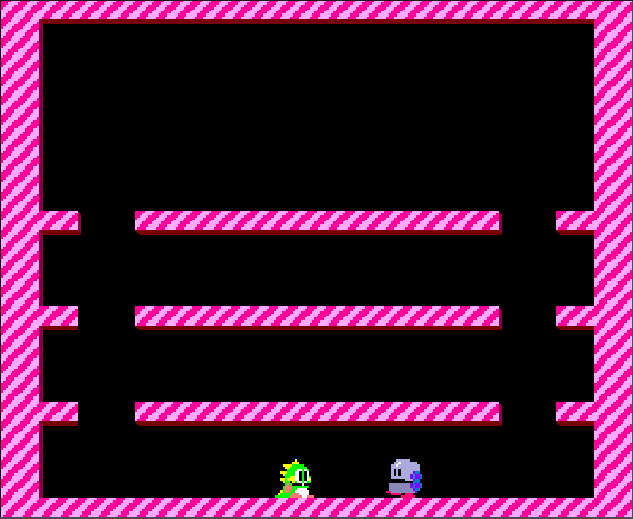
\includegraphics[scale=0.5]{media/gengner neben Spieler.png}
    \tiny\caption{Gegner Neben Spieler}
\end{figure}

\begin{figure}[h]
    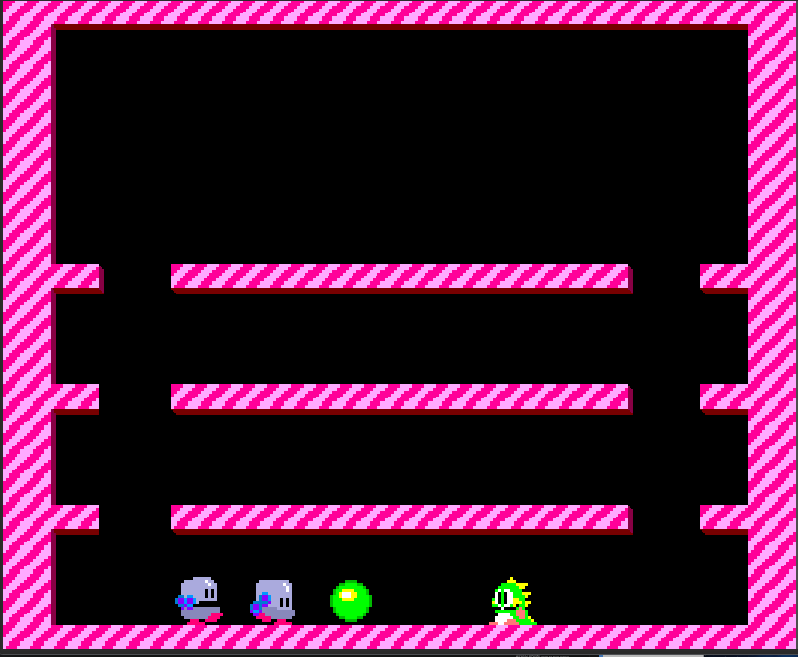
\includegraphics[scale=0.4]{media/Bildschirmfoto_20260605_194245.png}
    \tiny\caption{Spieler der Auf gegner Schießt}
\end{figure}


\section{Fazit}

Das Zeitmanagent war schlecht und Ziele zu groß.

\section{Quellen}

\end{spacing}
\end{document}